The basis of the confocal microscopy technique applied for the experiments in this thesis is fluorescence. Fluorescence is one type of photoluminescence which, in general, describes the emission of photons from a material after the absorption of light \cite{Lakowicz2006}. Photoluminescence occurs mostly for molecules with aromatic compounds such as benzene \cite{Li1972}. A profound understanding of photoluminescence requires an extensive quantum mechanical analysis. Therefore, this section only gives a phenomenological description.\\

Similar to the well-known particle in a box problem, the electrons in a molecule can take different energy levels that can be visualized in a Jablonski diagram, see Figure~\ref{fig:JablonskiDiagram}. The electronic energy levels are associated with molecular orbitals. They are denoted by S$_0$, S$_1$, and S$_2$ for singlet states and by T$_1$ for a triplet state. S$_0$ is the highest occupied molecular orbital in the ground state. Due to rotational and vibrational degrees of freedom for molecules, there are additional energy levels that further split up the electronic states. The electron in S$_0$ can be transferred into a higher electronic state by absorption of a photon with enough energy. The excited electron can be moved back to lower energetic states by non-radiative processes, where no photons are emitted. Another possibility is the direct transfer of the electron from S$_1$ to S$_0$ under the emission of a photon. This process is called fluorescence. A less likely path is the transition of the electron from S$_1$ into the triplet state T$_1$, called intersystem crossing. The transition from T$_1$ to S$_0$ under photon emission is called phosphorescence. Since it is in principle quantum mechanically forbidden, the lifetime of an electron in a triplet state is usually around \SI{e-6}{\second}. In comparison, the time that an electron remains in a particular singlet state lies at around \SI{e-9}{\second} \cite{Lichtman2005}.\\

\begin{figure}[h!]
	\centering
	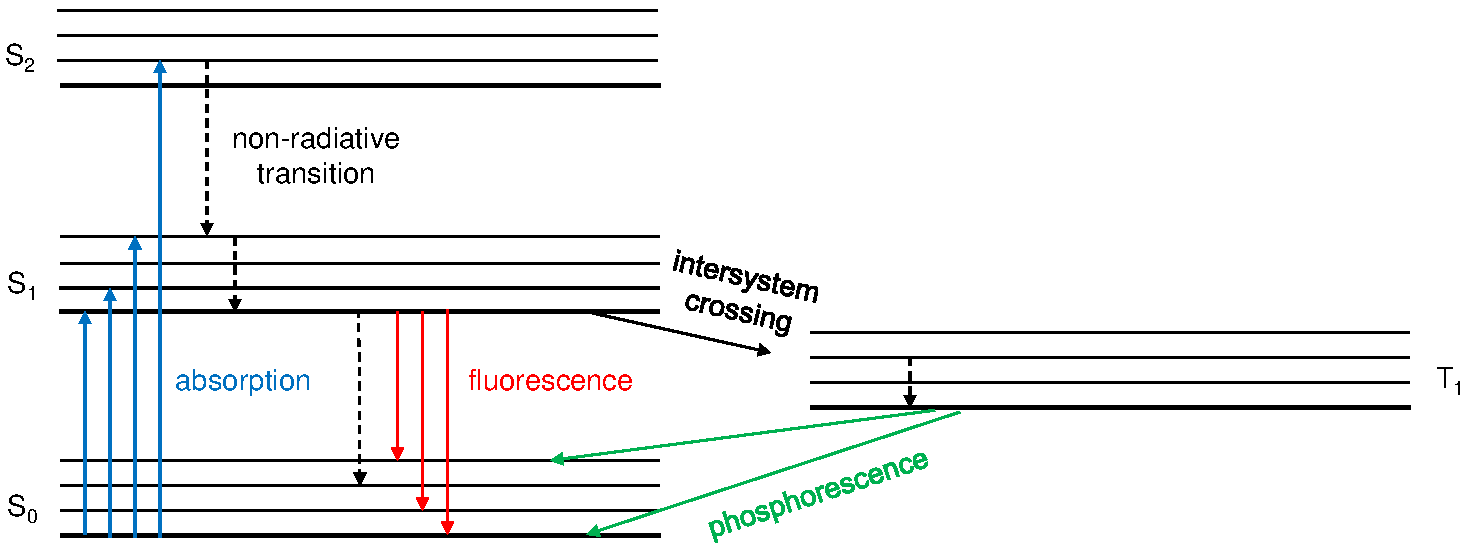
\includegraphics[width = 13cm]{JablonskiDiagram.pdf}
	\caption[Example of a Jablonski diagram]{Example of a Jablonski diagram. The different energy states and transition processes of an electron in a molecule are shown. S$_0$ is the highest occupied molecular orbital in the ground state.}
	\label{fig:JablonskiDiagram}
\end{figure}

A common way to classify a fluorophore is to measure its absorption and emission spectrum. The spectra are continuous due to the variety of energy states and transitions in a molecule (Figure~\ref{fig:JablonskiDiagram} shows only a few of them for illustration). An example of the red fluorescent dye Alexa 647 can be found in Figure~\ref{fig:Alexa647_Spectra}. In the figure, typical characteristics of the spectra of a fluorophore can be observed. First of all, the emission spectrum is shifted to higher wavelengths because before fluorescence occurs, the excited electron loses energy by non-radiative transitions. This effect is called Stokes shift and is an essential requirement for the functionality of a confocal fluorescence microscope since it allows to distinguish between incoming light and fluorescence light \cite{Lichtman2005}. Furthermore, the emission spectrum is a mirror image of the absorption spectrum because the vibrational and rotational energy states of the electronic states S$_0$ and S$_1$ have the same patterns. Finally, the emission spectrum is independent of the wavelength of the incoming light since fluorescence mostly occurs from the vibrational ground state of an energy level, e.g., from the ground state of S$_1$ \cite{Lakowicz2006}.

\begin{figure}[h!]
	\centering
	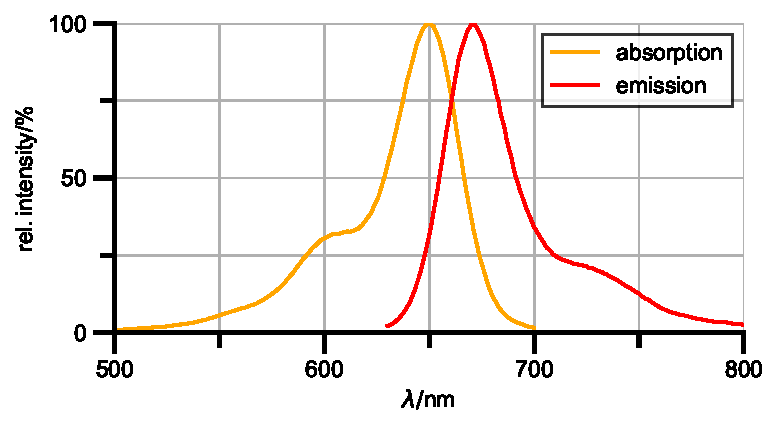
\includegraphics{Alexa647_Spectra.pdf}
	\caption[Absorption and emission spectrum of Alexa 647]{Absorption and emission spectrum of Alexa Fluor™ 647 (Thermo Fisher Scientific Inc., Waltham, USA) \cite{Alexa647_Spectra}. The intensity normalized on its maximum value is plotted against the wavelength $\lambda$.}
	\label{fig:Alexa647_Spectra}
\end{figure}